\startSolutions{outer}{Outer Products}

\begin{enumerate}[!HW!, start=1]
\item $\mtx{rr}{1&7\\7&2}$ (as long as the $(2,1)$ position is $7$, the values on the diagonal entries could be any real number).
\begin{multicols}{3}
\itemspade $\mtx{rrr}{1&2&3\\2&1&2\\3&2&1}$
\itemspade $\mtx{rrr}{7&8&9\\8&5&6\\9&6&3}$
\itemspade $\mtx{rrrr}{56&21&3&23\\21&91&85&75\\3&85&43&35\\23&75&35&62}$
\end{multicols}
\begin{multicols}{4}
\item $\mtx{ccccc}{1&6&8&9&13\\6&7&23&14&8\\8&23&11&16&19\\9&14&16&54&22\\13&8&19&22&72}$ (note that the $(1,1)$ position could be any real number) \columnbreak %Samuel Andersen
\item $\mtx{ccc}{1&7i&5-2i\\-7i&3&-9i\\5+2i&9i&2}$


\item $\mtx{rr}{1&2\\3&4}$
\item $\mtx{rrr}{1&2&3\\2&1&4\\3&5&1}$
\end{multicols}
\item $\mtx{rrrr}{1&2&3&4\\5&6&7&8\\9&0&1&2\\3&4&5&6}$

\begin{multicols}{4}
\itemspade Hermitian %NEW
\itemspade Hermitian %NEW
\itemspade not Hermitian %NEW
\itemspade Hermitian %NEW
\end{multicols}

\begin{multicols}{3}
\item $\mtx{rr}{0&-2\\2&0}$
\item $\mtx{rrrr}{0&3&9&3\\-3&0&5&-2\\-9&-5&0&-9\\-3&2&9&0}$


\itemspade$\mtx{rr}{-12&0\\8&0}$
\end{multicols}
\begin{multicols}{3}
\itemspade $\mtx{rrr}{8&-2&4\\-8&2&-4\\4&-1&2}$
\itemspade $\mtx{rr}{1&-3\\1&-3\\2&-6}$

\item $\bb u =\vr{7\\2\\1}, \bb v=\vr{-4\\0\\1}$
\end{multicols}
\begin{multicols}{3}
\item $\bb u = \vr{-2\\1\\4\\-1}, \bb v= \vr{-7\\2}$
\item $\bb u = \vr{3\\3\\6\\9\\4}, \bb v= \vr{2\\3\\2\\4}$
\item $\bb u = \vr{-9\\0\\0\\8}, \bb v= \vr{-2\\0\\0\\-5}$
\end{multicols}
\begin{multicols}{3}
\itemspade idempotent
\itemspade neither %nonsingular
\itemspade nilpotent
\end{multicols}

\itemspade \begin{multicols}{2} The projection of the unit square is the line segment between the points $(0,0)$ and $(1,1)$. As such, it has no area because it is only a line segment. The notion of area is lost by projections.
\begin{center}
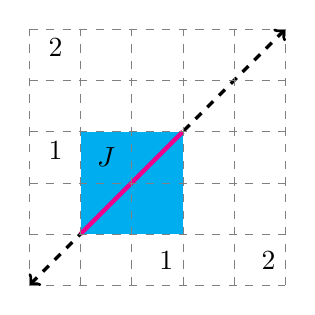
\begin{tikzpicture}[scale=0.65]
\fill[cyan] (0,0) rectangle (2,2);
\draw[dashed, very thick, <->] (-1,-1) -- (4,4);
\draw[, ultra thick, magenta] (0,0) -- (1,1) -- (2,2) -- (1,1) -- cycle;
%\fill[magenta!50!cyan] (0,0) rectangle (1,2);
\draw[help lines,dashed] (-1,-1) grid (4,4);
\node at (0.5,1.5) {$J$};
\begin{scope}[cm={0.5,0.5,0.5,0.5,(0,0)}]
\node[transform shape] at (1,1) {$J$};
\end{scope}
\gridlines{-1}{4}{-1}{4};
\node[below left, yshift=-3] at (2,0) {$1$};
\node[below left, yshift=-3] at (4,0) {$2$};
\node[below left, xshift=-3] at (0,2) {$1$};
\node[below left, xshift=-3] at (0,4) {$2$};
\end{tikzpicture}
\end{center}
\end{multicols}

\item \begin{enumerate}
    \item \begin{proof}
The result follows from the linearity of the transpose operator and $(A^\top )^\top  = A$:
\[(A+A^\top )^\top  = A^\top +(A^\top )^\top  =  A^\top  + A = A+A^\top . \qedhere\]
\end{proof}\vs 
    \item \begin{proof}
The result follows from the linearity of the transpose operator and $(A^\top )^\top  = A$:
\[(A-A^\top )^\top  = A^\top +((-A)^\top )^\top  =  A^\top  + (-A) = -A+A^\top  = -(A-A^\top ). \qedhere\]
\end{proof}

    \item \begin{proof}
Let $S = \dfrac{1}{2}(A+A^\top )$ and $T = \dfrac{1}{2}(A-A^\top )$. Then 
\[S+T = \dfrac{1}{2}(A+A^\top ) + \dfrac{1}{2}(A-A^\top ) = \dfrac{1}{2}(A+A) + \dfrac{1}{2}(A^\top -A^\top ) = \dfrac{2}{2}A + 0 = A.\] By part $(a)$, we know that $A+A^\top $ is symmetric. Since the transpose operator is linear, any scalar multiple of a symmetric matrix is symmetric. Thus, $S$ is symmetric. A similar argument using part $(b)$ shows that $T$ is skew-symmetric. Therefore, $A$ can be decomposed into a sum of symmetric and skew-symmetric matrices.
\end{proof}
\end{enumerate}

\item \begin{proof}
Let $A$ be an idempotent matrix, that is, $A^2=A$. Suppose that $A$ is also nonsingular. Then 
\[A^2 = A \qRightarrow A^{-1}(A^2) = A^{-1}(A)  \qRightarrow I_nA = I_n \qRightarrow A = I_n.\]

Suppose next that $A$ is nilpotent, that is, there exists some $m$ such that $A^m = 0$. Let $m$ be the smallest positive integer with this property. By the way of contradiction, suppose that $A$ is also nonsingular. Then 
\[A^m = 0 \qRightarrow A^{-1}(A^m) = A^{-1}(0)  \qRightarrow I_nA^{m-1} = 0 \qRightarrow A^{m-1} = 0.\] This contradicts the minimality of $m$. Therefore, $A$ cannot be nilpotent and nonsingular.
\end{proof}

\item We say that a square matrix $A$ is \textbf{skew-Hermitian} if $A^* = -A$. For example, the matrix $\mtx{ccc}{i & 3 & 4i\\ -3 & 0 & 1-2i \\ 4i & -1-2i & -7i}$ is skew-Hermitian.
\end{enumerate}

\vspace{-15 pt}